\documentclass{amsart}
\usepackage[margin=3cm]{geometry}                   % See geometry.pdf to learn the layout options. There are lots.
\geometry{letterpaper}                              % ... or a4paper or a5paper or ...
%\geometry{landscape}                               % Activate for for rotated page geometry
\usepackage[parfill]{parskip}                       % Activate to begin paragraphs with an empty line rather than an indent
\usepackage{float}
\usepackage{graphicx}
\usepackage{amssymb}
\usepackage{epstopdf}
\usepackage{siunitx}
\usepackage{subcaption}
\usepackage{units}
\usepackage{easytable}
\usepackage{setspace}
\usepackage{wrapfig}

\DeclareGraphicsRule{.tif}{png}{.png}{`convert #1 `dirname #1`/`basename #1 .tif`.png}

\title{X-Ray Diffraction}
\author{Caspar \textsc{Lant}} % Author name

\date{\today} % Date for the report

\begin{document}

\bigskip

\maketitle % Insert the title, author and date
\begin{center}

Intermediate Experimental Physics II\\
\vspace{1.5cm}

\begin{tabular}{l r}

Section: & 002\\
\\
Date Performed: & February 9, 2016 \\ % Date the experiment was performed
Date Due: & February 16, 2016\\
\\
Partner: & Neil Saddeler \\ % Partner names
Professor: & Prof. Andrew Kent\\
Instructor: & David Mykytyn % Instructor/supervisor
\end{tabular}
\end{center}
\vspace{50mm}
\pagebreak

\setstretch{1.3}
\paragraph{\textbf{The Objective} of this week's experiment was glean a glimpse into the atomic and structural composition of a couple elements, primarily with the aid of x-ray diffraction. }

\section{Theoretical Background/ Abstract}
\vspace{5pt}
\begin{figure}[H]
    \begin{minipage}{.35\textwidth}
        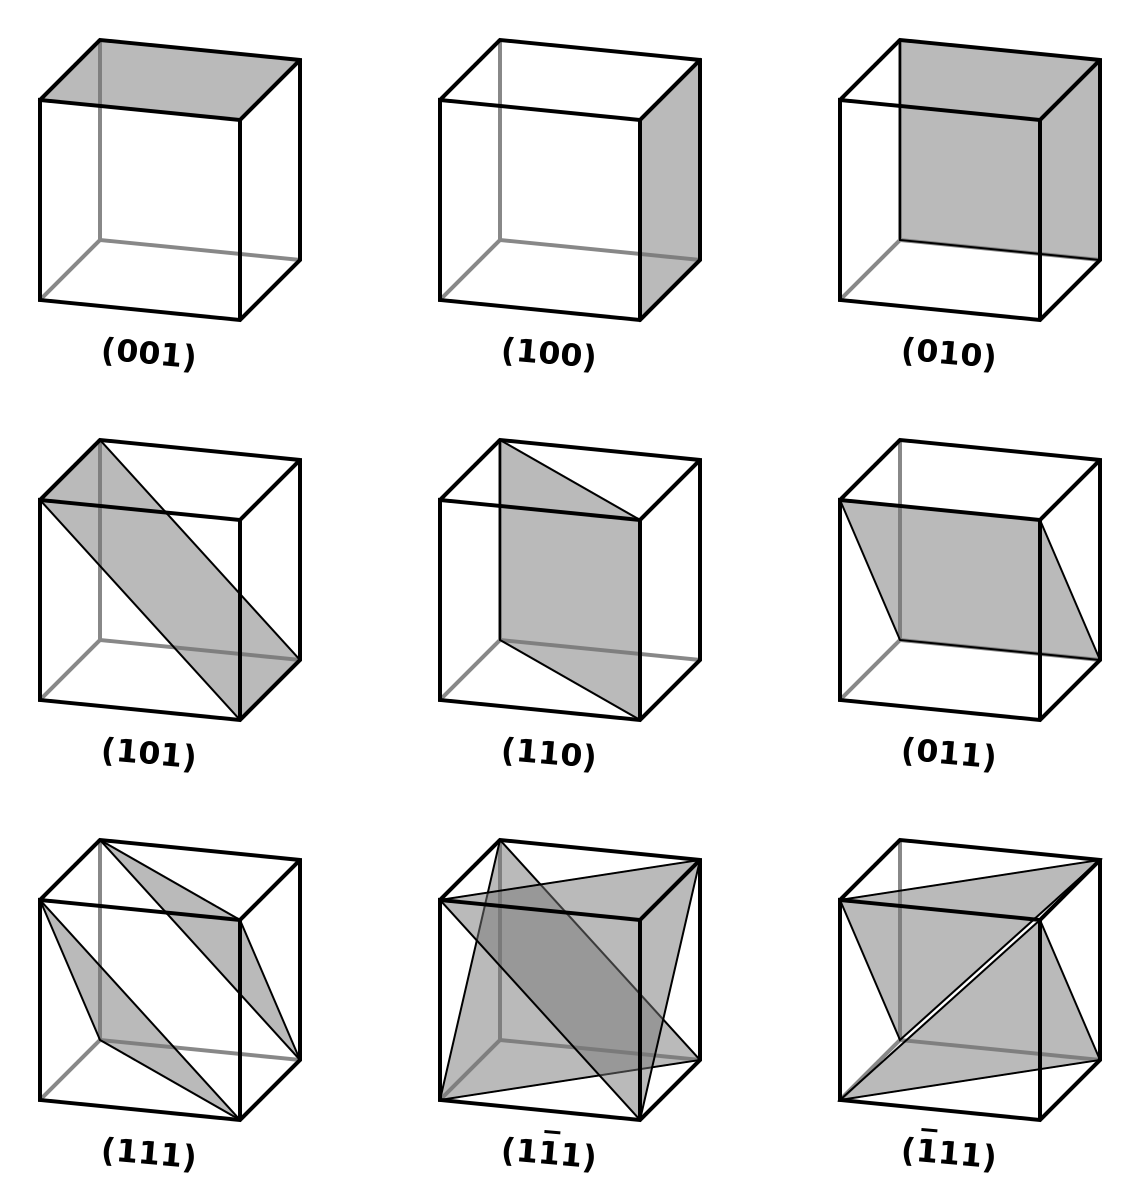
\includegraphics[width=0.96\textwidth]{Miller_Indices_Cubes.png}
        \caption{}
    \end{minipage}
    %
    \begin{minipage}{.63\textwidth}
        \setstretch{1.3}
        The structures of crystal latticies can be examined by using the techniques of x-ray crystallography, which extend from basic princibles of light diffraction. Cubic latticies present in materials like sodium chloride (table salt) and aluminum form parallel planes in regions of high atom-density (see figure 1). The most apparent planes (corresponding to regions of largest atom-density) are orthogonal to the lattice structure, and can be seen as ``extensions" of each cubic face. These orthogonal planes are seperated by what's referred to as the ``latice spacing" of the material. Bragg's law will help us calculate the lattice spacing of our samples:
    \end{minipage}
\end{figure}

\vspace{-.3cm}
\begin{figure}[H]
        \centering
        \[ \scalebox{1.5}{Bragg's Law: \hspace{5pt} $m\lambda = 2d\sin(\beta)$} \]
\end{figure}
\vspace{-.3cm}

Where $\beta$ is the angle of reflection, $\lambda$ is the wavelength of incident light, and $d$ is the lattice constant; the spacing between ``planes" in the material. $m=0,\pm1,\pm2,$ and so on. We may remember from our studies in optics that when light is incident on a material boundary between two media, some of it will reflect off the boundary, and the rest will pass through into the next layer, in a ratio that corresponds to the relative indeces of refraction of the two media. This effect is illustrated in the following diagram:
% \vspace{-1cm}
% 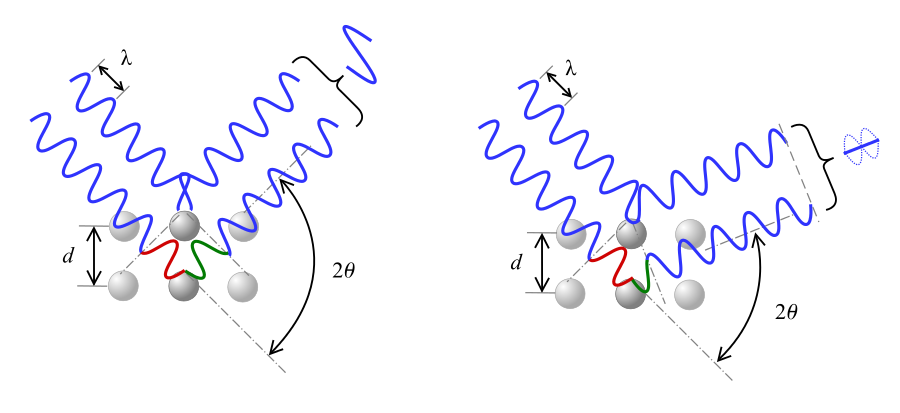
\includegraphics{bragg1.png}
\begin{figure}[H]
    \begin{minipage}{.5\textwidth}
        \centering
        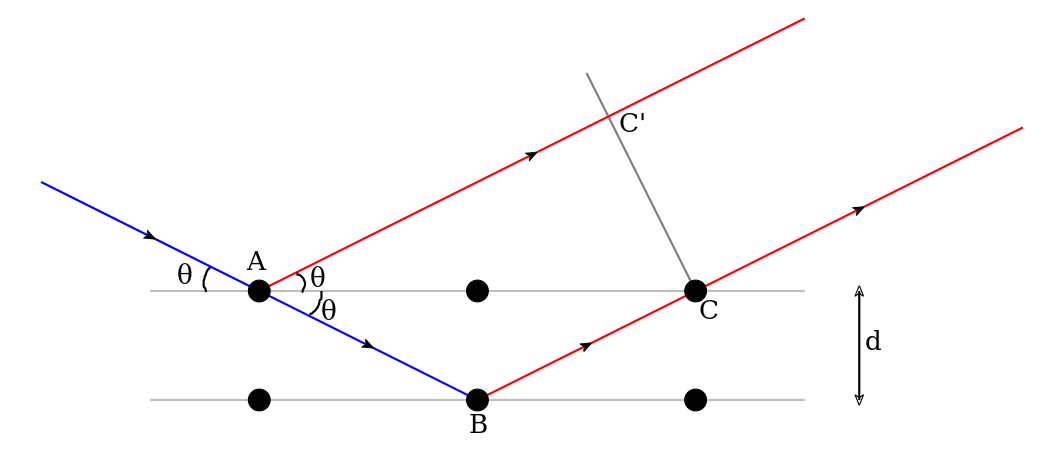
\includegraphics[width=\textwidth]{bragg2.png}
    \end{minipage}
    %
    \begin{minipage}{.47\textwidth}
        \setstretch{1.3}
        In this diagram, dots represent atoms, and the thin lines depict the planes that they form. Again, $d$ is the lattice constant. It's important to note that usually the lattice ``constant" seperated into distinct orthogonal components to account for non-cubic latticies, but in the case of Al and NaCl, $d$ is the same in all directions.
    \end{minipage}
\end{figure}

The energy of the electrons is given by the electron charge, $e^-$, time the voltage in the tube, which tends to be very high. This metric is also the energy of the emitted x-ray. This can be seen by extending the Planck-energy formula $E = h \nu$, where $h$ is the Plank constant, $\unitfrac[6.62 \times 10^{-34}]{m^2 kg}{s}$.
\vspace{5pt}
 \[E = e^-U = \dfrac{hc}{\lambda}\]

Mosley's Law, as shown on the right, gives us the wavelength and frequencies of the x-rays emmited from our tube. It just so happens that $n=2$ gives us $K_{\alpha}$, our lower-bound for frequency, and $n=3$ yeilds $K_{\beta}$, our upper bound. $R$ is the Rydberg constant, equal to $\unit[1.097 \times 10^{7}]{m^{-1}}$. Z is the atomic number of the x-ray-emitting material, which in this case is 42 (for Molybdenum).
\vspace{7pt}
\begin{table}[H]
    \begin{minipage}{.35\textwidth}
        \[\dfrac{1}{\lambda} = R\left(Z-1\right)^2 \left(1-\frac{1}{n^2}\right)\]
    \end{minipage}
    %
    \begin{minipage}{.6\textwidth}
        \renewcommand{\arraystretch}{1.1}
        \centering
        \begin{tabular}{@{}c|c|c|c|c@{}}
            $\unit[R]{(m^{-1})} $      & Z  & n & $\unit[\nu]{(Hz)}$  & $\unit[\lambda]{(m)}$ \\ \hline
            $1.10\times10^7$           & 42 & 2 & $1.38\times10^{10}$ & $7.23\times10^{-11}$  \\
            $1.10\times10^7$           & 42 & 3 & $1.64\times10^{10}$ & $6.10\times10^{-11}$  \\
        \end{tabular}
    \end{minipage}
\end{table}

\section{Experimental Procedure}
\begin{enumerate}
\item Plug the X-Ray machine into the power supply and turn it on.
\item Start the ``X-Ray Apparatus" software on the nearby compupeter.
\item Select USB Connection in the settings menu in the recently opened software
\item Open the righthand sliding door of the X-ray apparatus and place the collimator in the designated slot, located between the x-ray tube and the larger compartment. The collimator should click into place with satisfying precision.
\item Mount the geiger counter into the rotating arm about 10cm away from the sample podium. Tighten the thumpscrew and plug the bayonet connector into the signal jack.
\item Place the NaCl sample into the sample holder, and tighten another thumbscrew to hold it in place.
\item Close the righthand sliding door, and ensure that the lefthand door is fully closed. Don't worry, the machine will not start if either door is open.
\item Make sure that the step angle, step time, current, voltage, and minimim and maximum angles are set correctly.
\item Begin a run by pressing the `start' icon in the software interface.
\item Repeat the experiment with different values for voltage and current, and observe the effect.
\item Shield the measurement from certain frequencies with any of the supplied metallic filters.
\item When finished, repeat steps 6 though 11 for the aluminum sample.
\item If you still have the time/patience, remove the geiger counter, collimator, sample holder, and filter from the x-ray enclosure, and replace them an object of personal interest that you would like to have x-ray'd.
\item Remove the round panel from the right side of the machine, close the door, and perform a scan. It's possible\--but highly unlikely\-- that you'll see an image on the exposed phosphor sheet. This, ideally, would function in a manner similar to an oscilloscope.
\end{enumerate}

\renewcommand{\arraystretch}{1.1}
\section{Graphs and Calculations}

\begin{table}[H]
    \begin{minipage}{.25\textwidth}
        \centering
        \caption{NaCl}
        \vspace{13pt}
        \begin{tabular}{c|c}
            \# & $\beta^{\circ}$ \\ \hline
            1    & 6.3             \\
            2    & 7.2             \\
            3    & 14.8            \\
            4    & 22.1            \\
            5    & 26
        \end{tabular}
    \end{minipage}
    %
    \begin{minipage}{.7\textwidth}
            \centering
            \caption{Lattice Length}
            \label{my-label}
            \begin{tabular}{llll}
                $m=1$                               &               &$m=2$                              &               \\
                \multicolumn{1}{l|}{$d_{K_{\alpha}}$ \ meters}  & $d_{K_{\beta }}$ \ meters & \multicolumn{1}{|l|}{$d_{K_{\alpha}}$ \ meters} & $d_{K_{\beta }}$ \ meters\\ \hline
                \multicolumn{1}{l|}{$ 2.15 \times10^{-09}$}      & $ 1.81 \times10^{-09} $     & \multicolumn{1}{|l|}{$ 4.30 \times10^{-09}$}     & $ 3.63 \times10^{-09} $     \\
                \multicolumn{1}{l|}{$ 4.55 \times10^{-11}$}      & $ 3.84 \times10^{-11} $     & \multicolumn{1}{|l|}{$ 9.11 \times10^{-11}$}     & $ 7.68 \times10^{-11} $     \\
                \multicolumn{1}{l|}{$ 4.58 \times10^{-11}$}      & $ 3.87 \times10^{-11} $     & \multicolumn{1}{|l|}{$ 9.17 \times10^{-11}$}     & $ 7.74 \times10^{-11} $     \\
                \multicolumn{1}{l|}{$-3.33 \times10^{-10}$}      & $-2.81 \times10^{-10} $     & \multicolumn{1}{|l|}{$-6.65 \times10^{-10}$}     & $-5.61 \times10^{-10} $     \\
                \multicolumn{1}{l|}{$ 4.74 \times10^{-11}$}      & $ 4.00 \times10^{-11} $     & \multicolumn{1}{|l|}{$ 9.48 \times10^{-11}$}     & $ 8.00 \times10^{-11} $     \\
            \end{tabular}
    \end{minipage}
\end{table}

{\centering Bragg diffraction off of NaCl sample with X-Ray light within the wavelength of 61 to 72 pico meters}

\begin{figure}[H]
        \centering
        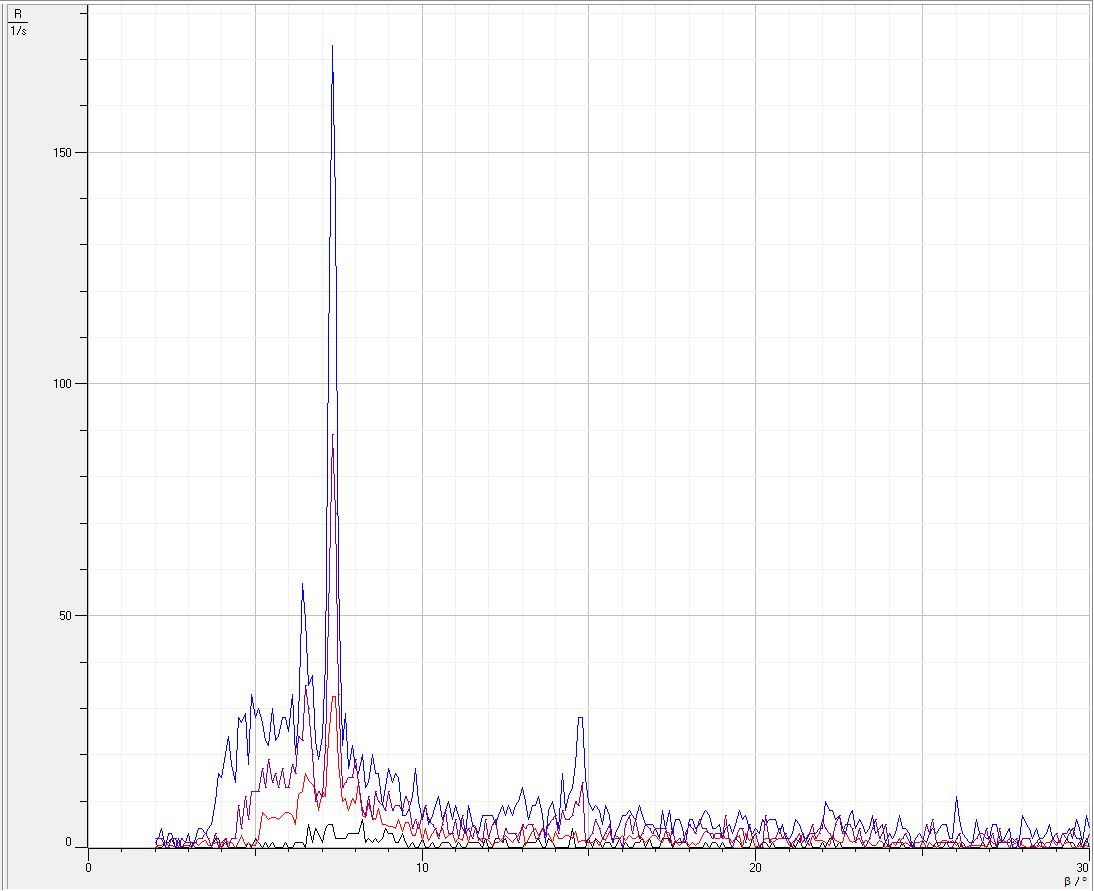
\includegraphics[width=\textwidth]{NaCl_all.PNG}
        \caption{Bragg Diffraction off NaCl at 20V, 25V, 30V, 35V}
\end{figure}


\begin{table}[H]
    \begin{minipage}{.25\textwidth}
        \centering
        \caption{Al}
        \vspace{13pt}
        \begin{tabular}{c|c|c}
            \# & $\unit[\beta]{^\circ}$ & \unitfrac[R]{(1}{s)}  \\ \hline
            1  & 7.3             & 180 \\
            2  & 8.4             & 390 \\
            3  & 9.7             & 75  \\
            4  & 15.2            & 41  \\
            5  & 17.4            & 104 \\
            6  & 26.8            & 29  \\
        \end{tabular}
    \end{minipage}
    %
    \begin{minipage}{.7\textwidth}
            \centering
            \caption{Lattice Length}
            \label{my-label}
            \begin{tabular}{llll}
                $m=1$                              &               &$m=2$                               &               \\
                \multicolumn{1}{l|}{$d_{K_{\alpha}}$  meters} & $d_{K_{\beta }} $  meters  & \multicolumn{1}{|l|}{$d_{K_{\alpha}}$  meters}& $d_{K_{\beta }}$  meters\\ \hline
                \multicolumn{1}{l|}{$ 4.25\times10^{-11}$}      & $ 3.59\times10^{-11}$     & \multicolumn{1}{|l|}{$ 8.50\times10^{-11}$}    & $ 7.17\times10^{-11}$     \\
                \multicolumn{1}{l|}{$ 4.23\times10^{-11}$}      & $ 3.57\times10^{-11}$     & \multicolumn{1}{|l|}{$ 8.46\times10^{-11}$}    & $ 7.14\times10^{-11}$     \\
                \multicolumn{1}{l|}{$-1.33\times10^{-10}$}      & $-1.12\times10^{-10}$     & \multicolumn{1}{|l|}{$-2.66\times10^{-10}$}    & $-2.24\times10^{-10}$     \\
                \multicolumn{1}{l|}{$ 7.43\times10^{-11}$}      & $ 6.27\times10^{-11}$     & \multicolumn{1}{|l|}{$ 1.49\times10^{-10}$}    & $ 1.25\times10^{-10}$     \\
                \multicolumn{1}{l|}{$-3.64\times10^{-11}$}      & $-3.07\times10^{-11}$     & \multicolumn{1}{|l|}{$-7.28\times10^{-11}$}    & $-6.14\times10^{-11}$     \\
                \multicolumn{1}{l|}{$ 3.63\times10^{-11}$}      & $ 3.06\times10^{-11}$     & \multicolumn{1}{|l|}{$ 7.26\times10^{-11}$}    & $ 6.13\times10^{-11}$
            \end{tabular}
    \end{minipage}
\end{table}

{\centering Bragg diffraction off of Al sample with X-Ray light within the wavelength of 61 to 72 pico meters}
\begin{figure}[H]
    \centering
    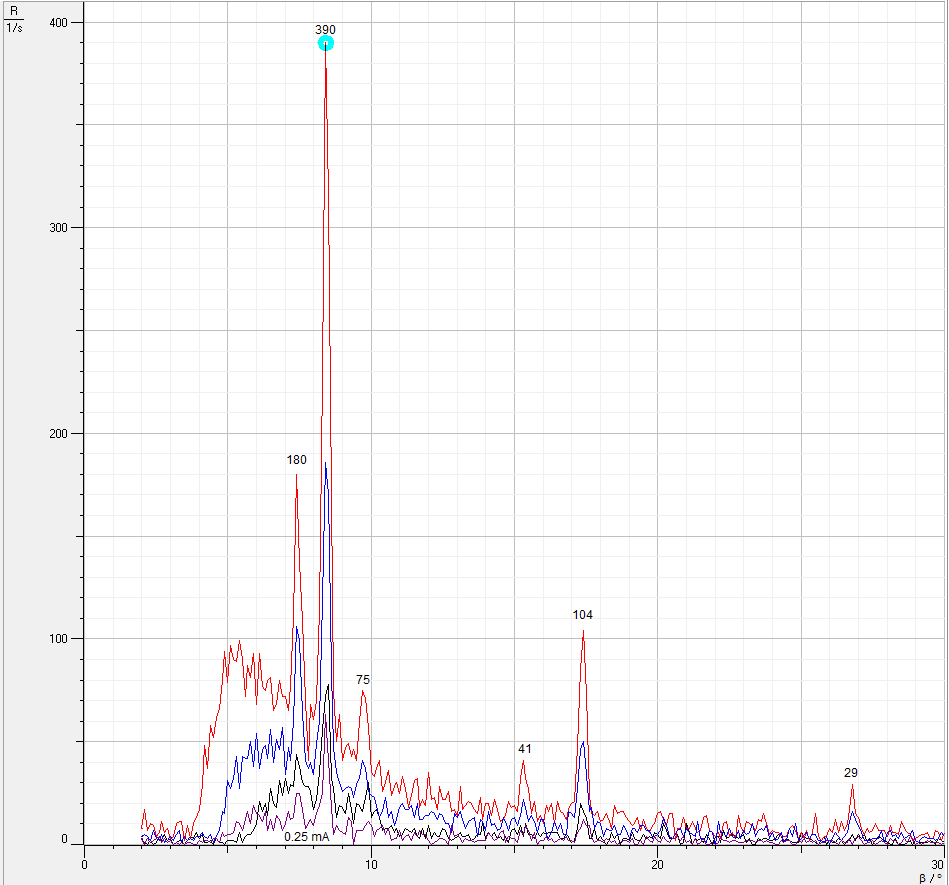
\includegraphics[width=\textwidth]{Al_annotations.PNG}
    \caption{Bragg Diffraction off Aluminum Sample at 20V, 25V, 30V, 35V, and 0.25mA}
\end{figure}

\section{Questions}

\setstretch{1}

\begin{enumerate}
\item {\textit{The maximum energy xray depends on U (see above), in fact $\lambda_{min}={hc}/{U_{e^-}}$. Find the minimum beta (maximum xray energy) for each run and plot $\sin(\beta)$ vs. ${hc}/{2U_{e^-}}$ to find the value for $d$ for NaCl.}
\begin{quote}
The lattice constant for NaCl is shown in the table above. It seems to be between 400 and 600 picometers $(10^{-12} \ \text{meters})$.
\end{quote}}


\item {\textit{Take similar runs with the Al crystal sample and perform the same analysis steps. How does the value for d compare? Do the wavelengths of the K peaks change?}
\begin{quote}
The lattice contast for Aluminum is between 359 and 425 picometers, which is slightly less than our values for sodium chloride. Yes, the wavelengths change.
\end{quote}}

\item {\textit{Change the current used to 0.75, or 0.5, or 0.25 mA and repeat the Al run with U=35kV. What's the effect and what stays the same? Explain.}
\begin{quote}
The location of peaks say the same, height of them decreases with decreasing current (see figure 4).
\end{quote}}

\item {\textit{What happens at even smaller angles than 2 degrees?}
\begin{quote}
At diffraction angles smaller than 2 degrees, the geiger counter feels the full brunt of the beam. The reason these angles are exclluded is because they ``wash out" the rest of our measurements.
\end{quote}}

\item{\textit{What happens when adding xray filters such as Zr, Cu, Mo, Ag?}
\begin{quote}
Cu blocked all diffracted x-rays.
\end{quote}}

\item{\textit{What if you remove the collimator?}
\begin{quote}
See attached.
\end{quote}}

\end{enumerate}

\section{Error Analysis}
Our main sources of error were in the measurement of the angles of diffraction. Because I did this by eye, I'd say that each measurement is accurate to within one half of a degree. I could have mitigated this error by exporting my data, and parsing for the angle at which each peak occurs. In general, an automated approach will produce less error than one that I am heavily implicated in. My degree of uncertainty in lattice length is given by the following formula, and tend to be on the scale of picometers for the aluminum and sodium chloride samples. These measurements are two orders of magnitude less than the calculated and expected values for lattice length. Our main sources of error were in the measurement of the angles of diffraction. Because I did this by eye, I'd say that each measurement is accurate to within one half of a degree. I could have mitigated this error by exporting my data, and parsing for the angle at which each peak occurs. In general, an automated approach will produce less error than one that I am heavily implicated in. My degree of uncertainty in lattice length is given by the following formula, and tend to be on the scale of picometers for the aluminum and sodium chloride samples. These measurements are two orders of magnitude less than the calculated and expected values for lattice length.
\vspace{-0.2cm}
\begin{figure}[H]
    \begin{minipage}{0.3\textwidth}
        \[\delta d \ = \ |d|\sqrt{\left(\dfrac {\delta \beta }{|\beta|}\right)^2 + \left(\dfrac{\delta \lambda}{|\lambda|}\right)^2} \ \ \ \ \ \ \ \ \ \ \]
    \end{minipage}
    %
    \begin{minipage}{0.65\textwidth}
        I'd say that, given the magnitude of our measurements for uncertainty, our data is reliable enough to report on the lattice contant for the materials under scrutiny, with precision at the level of at least their physical scale. That is to say that the lattice length for Al is around 400pm, and is roughly 500pm for sodium chloride.x`
    \end{minipage}
\end{figure}


\end{document}
